Impedance Microbiology (IM) \cite{stewart1899charges} is a laboratory-technique used by microbiologist to establish the microbial number density of a sample. Its founding principle is that the metabolism of microorganisms transforms uncharged or weakly charged compounds present in the growth medium (such as sugars and proteins/peptides) into highly charged ones (carbon dioxide, organic acids, hydrogen ions, etc.). By monitoring the electrical properties of the culture broth, it is then possible to infer in real time the changes happening in its bacterial concentration: the growth in number of the microbial population corresponds to an increase in the produced metabolites, thus in the medium’s conductivity \cite{Grossi2017,Kargupta2018,Xu2016}. Again, this technique only teaches about the bacterial population, and not the individual bacteria. \par

The growth phases of bacterial colonies generally follow three growth steps, which can be associated with the change in conductivity of the growth medium, as illustrated in \autoref{fig:GrowthPhase}. An initial lag phase, in which the bacteria prepare for duplication is characterized by a low constant conductivity; the log phase, when the bacterial growth is maximal, can be retraced when the bacterial concentration reaches the critical microbial concentration threshold $C_{TH}$; the stationary phase, when the bacteria have depleted the nutriments in the medium, can be deduced by the halt of the conductivity after the log phase; the dead phase follows when the bacteria dies per lack of nutriment, and is the only phase that cannot be deduced by the medium’s conductivity since the highly charged compounds that now occupies the medium do not vanish after the death of the bacteria. Information about the life cycle can be used to differentiate between bacterial population since these characteristics are unique to each specie \cite{Sylvain2018}. 
\begin{figure}[h]
    \centering
    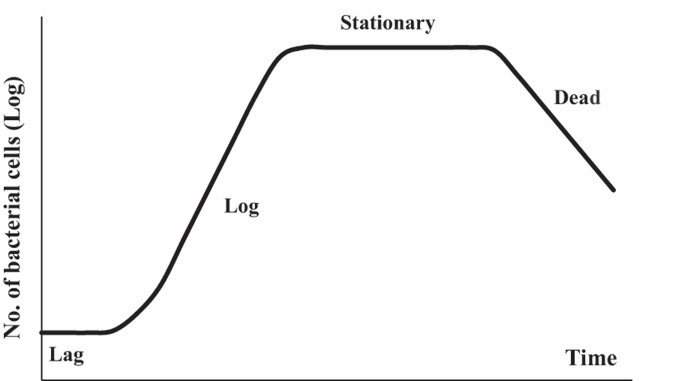
\includegraphics[width=0.7\textwidth]{GrowthPhase}
    \caption{Growth phases of a bacterial population.\citep{wang2015bacterial}}
    \label{fig:GrowthPhase}
\end{figure}

The first step in IM is to add an aliquot of the substance of interest (blood, sputum, food, specific microbe, yeast, etc.) to a chosen culture broth, while maintaining external conditions at a constant level suitable for an optimum growth of the target microorganisms. From there, the microorganisms, if present in the sample, will metabolize the compounds of the culture broth, which will modify the properties of the medium, such as pH, O2/CO2 levels, and electrical conductivity \cite{Kargupta2018,Xu2016}. In IM, it is the electrical conductivity which is monitored regularly as a function of time, generally by measurements of the complex impedance of the sample. The measured conductivity starts at a low baseline value and suddenly increases after a critical microbial concentration threshold $C_{TH}$ (in the range of 106-107 cfu/ml for cells in suspensions \cite{Xu2016,Lei2014}) is reached, which depends on the type of bacteria, electrodes, and culture broth chosen for the test. Since bacteria replication through binary fission is completed in a fixed time, it is then possible to deduce the initial microbial concentration $C_0$ of a sample by noting the Detect Time ($DT$) needed to attain the critical microbial concentration that significantly increases the conductivity. Seeing that DT is a linear function of the logarithm of the initial concentration, that value can be easily deduced \cite{Grossi2009,Xu2016}:
\begin{equation}
DT = A \log(C_0) + B
\end{equation}
\begin{equation}
C_0 = 10^{\frac {DT-B}{A}}
\end{equation}
Here, $A$ and $B$ are parameters that vary accordingly to the type of bacteria and culture broth chosen for the experiment, as well as some environmental conditions such as pH and temperature. They can be deduced with a calibration using bacteria and broth with known initial concentration and $DT$ in a supervised environment, followed by an adequate linear regression \cite{stewart1899charges}. \par